\pagestyle{empty} % Limpa o cabeçalho e o rodapé
\onehalfspacing % Espaçamento entre-linhas de 1,5
% \hyphenpenalty=10000 % To prevent hyphenation
\pretolerance=10000 % To avoif overful lines
%\selectlanguage{english}
\setcounter{ex}{0} % counter for exercises
\selectlanguage{brazilian}
%\pagenumbering{arabic} % Uncomment this line if you want renumber pages for each chapter
\renewcommand{\chaptername}{Tutorial}
\chapter{TNT - Buscas Avançadas}\label{tut5}
\rhead{\tiny Instituto de Biociências --USP: BIZ0433 - Inferência Filogenética: Filosofia, Método e Aplicações}
\cfoot{\tiny \cc \ccby \ccsa \href{http://creativecommons.org/licenses/by-sa/4.0/}{Creative Commons Attribution-ShareAlike 4.0 International License}}
%\vspace{5pt}
{\large \sc BIZ0433 - Inferência Filogenética: Filosofia, Método e Aplicações.}\par
%\vspace{10pt}
\par
\minitoc % for table of contents within the chapter
\newpage
\section*{}\addcontentsline{toc}{section}{Objetivo}
\onehalfspacing
\vspace*{5pt}
\begin{center}
\emph{\begin{large}Objetivo\end{large}}\label{tut5:Objetivo}
\vspace{2pt}
\end{center}
%% TEXTO DO RESUMO
Este tutorial visa apresentar as ferramentas mais avançadas de busca em TNT. Estas ferramentas são os algoritmos mais poderosos de TNT e garantem a esse programa muita eficiência em explorar o espaço de árvores, especialmente em bancos de dados complexos (\textit{i.e.}, grande número de terminais e caracteres). O tutorial explica brevemente os métodos implementados em TNT. No entanto, o componente teórico contido neste tutorial é superficial e o estudante é encorajado a consultar a literatura primária citada neste documento. Este tutorial também contém exercícios sobre reconstrução de estados ancestrais em topologias, bem como os comandos associados à diagnose de grupos em TNT. Eles são importantes para que o estudante tenha conhecimento de como explorar evolução de caracteres, bem como identificar os caracteres que sustentam grupos em sua análise usando este aplicativo. Os arquivos associados a este tutorial estão disponíveis no \href{https://github.com/fplmarques/cladistica/tree/main/tutorials/}{GitHub}. Você baixar todos os tutoriais com o seguinte comando:

\begin{center}
\small \texttt{svn checkout https://github.com/fplmarques/cladistica/trunk/tutorials/}\\
\end{center}

\newpage
\pagestyle{fancy} % Inclui o cabeçalho definido no meta.tex
%\pagenumbering{arabic} % Números das páginas em arábicos
\begin{refsection}
\renewcommand*{\finalnamedelim}{\addspace\&\space}% Usar '&' ao invés de 'e'.

%%%%%%%%%%%%%%%%%%%%%%%%%%%% HERE TEXT STARTS %%%%%%%%%%%%%%%%%%%%%%%%%%%% 
\section{Buscas com novas tecnologias}\label{tut5:newtech}

A maior vantagem do TNT \parencite{GoloboffEtAl_2008} em comparação a muitos programas de inferência filogenética é a rapidez com a qual este aplicativo executa buscas. Parte da velocidade do TNT está no código de execução de tarefas, mas há um outro componente que é resultado da implementação de novos algoritmos de buscas \parencite{Goloboff_1999, Nixon_1999}. No tutorial anterior vimos como as buscas tradicionais são feitas por algoritmos que começam com a construção de árvores de Wagner e subsequente refinamento por \textit{branch swapping} (\textit{i.e.}, RAS+SPR e/ou TBR, veja Tutorial \ref{tut4}, seção \ref{tut4:search}). Estas estratégias de busca por trajetórias são considerados ''\textit{Hill-climbing algorithms}'' uma vez que eles departem de uma topologia inicial em direção a outra melhor utilizando rearranjos internos (\textit{i.e., intra-tree branch swapping}, veja \textcite{Giribet_2007} e \textcite{Goloboff_1999}). Como pôde ser visto no tutorial anterior, esses algoritmos possuem limitações, principalmente em espaços de árvores complexos, pois eles podem restringir suas buscas a áreas nas quais se encontram apenas ótimos locais.

\subsection{Perturbações:}

De acordo com \textcite{Giribet_2007}, uma das estratégias mais inovadores de busca utilizando os algoritmos de rearranjos internos disponíveis naquele momento foi a técnica de \textit{ratchet} proposta por \textcite{Nixon_1999}. Esta técnica de aceleração de buscas heurísticas está implementada em TNT. A técnica de \textit{ratchet} usa ciclos de perturbações no espaço de topologias atribuindo pesos diferenciais à parte dos dados na expectativa de que a busca saia de ótimos locais (Figura \ref{tut5:fig:ratchet}). Nesse algoritmo, uma topologia é criada e refinada pelos algoritmos convencionais (\textit{i.e.}, RAS+TBR), ao término do rearranjo uma porcentagem dos dados recebe pesagens diferenciais, um novo ciclo de rearranjos é iniciado, após sua conclusão os caracteres voltam à pesagem original e o custo da topologia é avaliado. Se há mais ciclos a serem executados, esses passos são repetidos, caso contrário o custo da topologia resultante é comparado com a topologia inicial (Figura \ref{tut5:fig:ratchet}).

\subsection{Buscas setoriais:}

Outro conjunto de algoritmos disponíveis em TNT para explorar espaços de árvores mais complexos são aqueles destinados à buscas setoriais (\textit{sectorial search}, senso \textcite{Goloboff_1999}). Como o próprio nome indica, estes algoritmos -- conhecidos como algoritmos da família ``\textit{divide and conquer}'' -- reduzem a dimensão do espaço de soluções restringindo o problema à subconjuntos de problemas menores. No caso de buscas filogenéticas, o algoritmo implementado em TNT seleciona um setor (\textit{i.e.}, clado) da topologia que é reanalisado. Se uma configuração melhor é encontrada para esse clado, ele é substituído na topologia original (para maiores detalhes veja \textcite{Goloboff_1999, Wheeler_2012}). Os ciclos de iterações desse algoritmo está representado na Figura \ref{tut5:fig:secsearch}.


%%%%%%%%%%%%%%%%%%%%%%%%%%% FIGURA RATCHET %%%%%%%%%%%%%%%%%%%%%%%%%%%
%  \vspace{-1em}
  \begin{figure}[H]
    %\ffigbox[\FBwidth]
       \centering
      {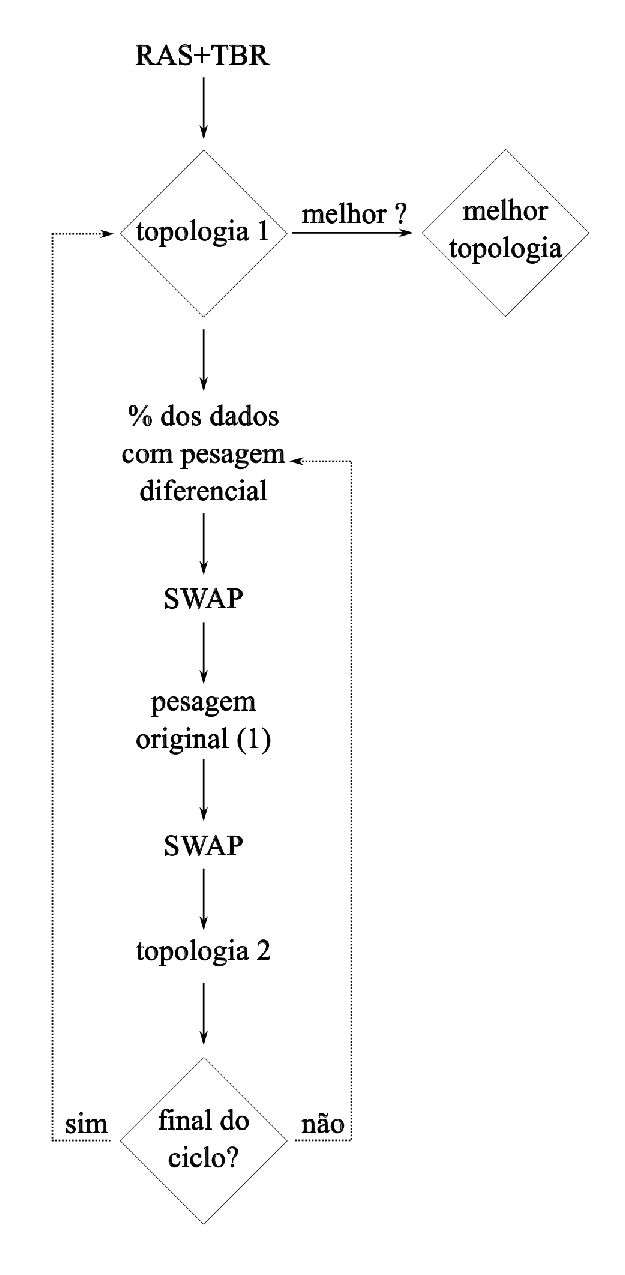
\includegraphics[scale=0.80]{figures/tut5/ratchet.eps}}
	{\caption[Fluxo de iterações de \textit{ratchet}]{Fluxo de iterações de \textit{ratchet}. \textbf{RAS}, \textit{radom addition sequence}; \textbf{SWAP}, \textit{branch swapping} via SPR ou TBR. Pesagem diferencial geralmente entre 5 e 10\% dos caracteres. Número de ciclos (\textit{k}) variável.}\label{tut5:fig:ratchet}}
  \end{figure}

%%%%%%%%%%%%%%%%%%%%%%%%%%% FIM DA FIGURA RATCHET %%%%%%%%%%%%%%%%%%%%%



%%%%%%%%%%%%%%%%%%%%%%%%%%% FIGURA SECTORIAL SEARCHES %%%%%%%%%%%%%%%%%%%%%%%%%%%
%  \vspace{-1em}
  \begin{figure}[H]
    %\ffigbox[\FBwidth]
       \centering
      {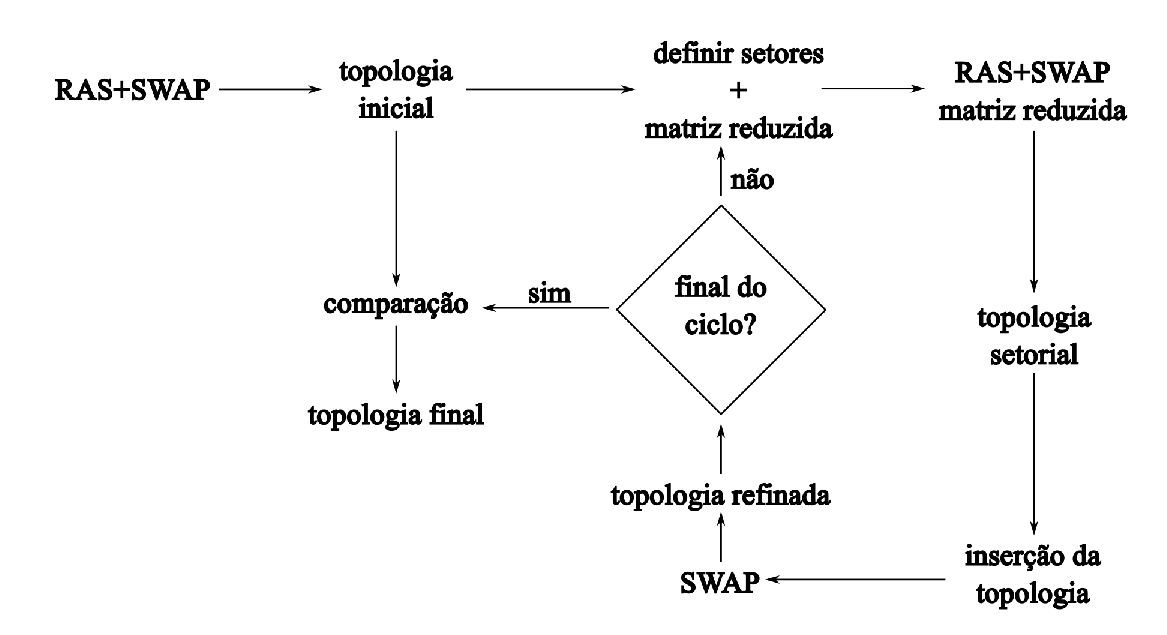
\includegraphics[scale=0.80]{figures/tut5/sectorial_search.eps}}
	{\caption[Fluxo de iterações de buscas setoriais.]{Fluxo de iterações de buscas setoriais de acordo com \textcite{Goloboff_1999}.}\label{tut5:fig:secsearch}}
  \end{figure}

%%%%%%%%%%%%%%%%%%%%%%%%%%% FIM DA FIGURA SECTORIAL SEARCHES %%%%%%%%%%%%%%%%%%%%%


\subsection{Annealing \& algoritmos genéticos:}

Dentro das novas tecnologias de busca de TNT há dois outros algoritmos que merecem consideração. O primeiro deles é o \textit{tree-drift}. Parte de métodos conhecidos como \textit{simulated annealing}, o \textit{tree-drift} é caracterizado por aceitar certa proporção de topologias subótimas durante o processo de rearranjo interno (\textit{i.e., swap}) alternado com a configuração original do \textit{swap}. Posteriormente, como em \textit{ratched}, topologias subótimas são descartadas e uma nova iteração do ciclo se inicia. Tais ciclos, que se repetem por um número determinado de vezes, são quase tão eficientes como o \textit{ratchet} na busca de topologias ótimas.

O segundo deles é o \textit{tree-fusing}. O \textit{tree-fusing} pertence a uma classe de algoritmos conhecidos como \textit{genetic algorithms}, pois ao contrário dos algoritmos ilustrados acima -- que baseiam-se em uma única topologia --, algoritmos genéticos promovem rearranjos de clados entre topologias. Implementado em TNT, esse método compara diferentes topologias e promove a troca de clados compatíveis (\textit{i.e.}, mesma composição entre as topologias). Esse método leva a melhores resultados quando há um número grande de topologias disponíveis para a troca. Para maiores detalhes sobre o método consulte \textcite{Giribet_2007, Goloboff_1999}.\\


\stepcounter{ex}
\begin{blackBlock}{\textbf{Exercicio 5.\arabic{ex}}}\label{tut4:ex:5.1}
No Tutorial \ref{tut4} fizemos uma série de buscas no arquivo \texttt{zilla.tnt} utilizando os algoritmos tradicionalmente implementados em programas filogenéticos (\textit{i.e.}, \textit{random addition sequence}, RAS ou árvore de Wagner, seguidas de refinamento por algoritmos de \textit{swap}, tais como SPR e TBR) para buscas heurísticas. Vocês devem ter observado que muito provavelmente ninguém obteve 100 topologias ao custo de 16218 passos. Neste tutorial iremos explorar a eficiência dos algoritmos descritos acima e verificar se de fato ele possibilitam um melhor resultado com a análise da matriz em \texttt{zilla.tnt}.
\end{blackBlock}

\begin {myindentpar}{0.3cm}
\begin{enumerate}[\itshape i.]

	\item{Configuração de \textit{default} do comando XMULT.}\\
	As buscas com novas tecnologias são implementadas no TNT pelo comando \texttt{xmult}, ou \texttt{xmu}. 
	  \begin {myindentpar}{0.5cm}
	  \begin{enumerate}[\itshape a.]
		\item{Abra o arquivo \texttt{zilla.tnt} no TNT}.
		\item{Execute o comando \texttt{xmu;} no TNT}.
		\item{Qual o custo da topologia que você encontrou e quantas topologias você recuperou?}
			\begin{center}
			\line(1,0){400}\\
			\end{center}
		\item{Qual foi a redução de custo desta topologia em comparação com sua melhor análise de \texttt{zilla.tnt} no Tutorial \ref{tut4}, Exercício \ref{tut4:ex:4.9}?}
			\begin{center}
			\line(1,0){400}\\
			\end{center}
		\item{Utilizando o comando \texttt{xmu:;} e o arquivo \texttt{xmu.txt} -- que contém o \textit{log} do comando \texttt{help xmu} --, escreva abaixo quais foram os parâmetros de execução do comando \texttt{xmu;} executado acima?}
			\begin{center}
			\line(1,0){400}\\
			\line(1,0){400}\\
			\line(1,0){400}\\
			\end{center}
	  \end{enumerate}
	  \end{myindentpar}

	\item{Modificando as Configurações de \textit{default} do comando XMULT.}\\
Nesse exercício iremos explorar como os diferentes algoritmos implementados no comando \texttt{xmu} modificam sua performance. Você deverá realizar seis análises, uma utilizando os algoritmos tradicionais de busca em TNT e as demais implementando sequencialmente os algoritmos mais agressivos sob o comando \texttt{xmu}. Os resultados dessas análises deverão ser anotados na Tabela \ref{tut5:table:xmu}. O arquivo \texttt{xmu.txt} deverá ser consultado caso tenha dificuldades de visualizar todas as opções do comando \texttt{xmu} na tela do terminal onde o TNT será executado. O arquivo que contém a matriz de \texttt{zilla.tnt} foi modificado para que o TNT utilize 512 MB de RAM e possa guardar 10000 topologias. Considere verificar os parâmetros de \texttt{xmu} à cada etapa do exercício para certificar-se de que os parâmetros que deseja estão de fato implementados.

 \begin {myindentpar}{0.3cm}
  \begin{enumerate}[\itshape a.]
   \item{Faça uma busca convencional em TNT utilizando 100 réplicas para adições aleatórias (\textbf{RAS}) e mantendo 10 topologias durante cada réplica para a matriz de \texttt{zilla.tnt}. Os resultados dessa análise deverão ser inseridos na Tabela \ref{tut5:table:xmu}.}
    \item{Utilizando 20 réplicas e a manutenção de 10 topologias por réplicas -- que deverá ser implementado em \texttt{xmu} (\textit{e.g.}, \texttt{xmu: rep 20 hold 10}) -- execute uma análise utilizando a configuração para o comando \texttt{xmu} que implemente \textbf{apenas buscas setoriais}. Observe que por \textit{default}, o TNT executa o comando \texttt{xmu} com os algoritmos de \textit{sectorial searches} e \textit{tree-fusing}. Desta forma você deverá desabilitar a execução do \textit{tree-fusing}. O arquivo \texttt{xmu.txt} -- que contém o \textit{log} do comando \texttt{help xmu} -- deverá ser consultado caso tenha dificuldades de visualizar todas as opções do comando \texttt{xmu} na tela. Os resultados dessa análise deverão ser inseridos na Tabela \ref{tut5:table:xmu}.}
    \item{O TNT utiliza concomitantemente duas estratégias de buscas setoriais implementadas nos algoritmos CSS (\textit{constraint-based sector selections}) e RSS (\textit{random sector selections}). Nesta execução de TNT nós queremos avaliar a performance do \textit{ratchet}. Desta forma você deverá desabilitar as buscas setoriais, implementar 10 iterações de \textit{ratchet}, executar a análise e registrar os resultados na Tabela \ref{tut5:table:xmu}.}
    \item{Excecute \texttt{xmu} implementando 10 ciclos de \textit{drift} e registre os resultados na Tabela \ref{tut5:table:xmu}. Certifique-se de que somente o \textit{drift} está habilitado.}
    \item{Excecute \texttt{xmu} implementando \textit{fuse} para ao conjunto de árvores e registre os resultados na Tabela \ref{tut5:table:xmu}. Certifique-se de que somente o \textit{fuse} está habilitado.}
    \item{Finalmente, você deverá implementar todos os algoritmos que executou acima e suas respectivas configurações em uma única análise e registrar os resultados na Tabela \ref{tut5:table:xmu}.}

  \end{enumerate}
 \end{myindentpar}
%%%%%%%%%%%%%%%%%%%%%%%%%%% TABELA DE PARA BUSCAS COM NEW TECHS %%%%%%%%%%%%%%%%%%%%%%%%%%% 
%\begin{landscape}
\pagestyle{fancy}
\begin{center}

\begin{longtable}{|c|c|c|c|c|c|c|}
\caption[Tabela \ref{tut5:table:xmu}: Buscas heurísticas com novas tecnologias em TNT]{Número de sequências aleatórias (\textbf{RAS}), topologias mantidas em cada réplica, algoritmo implementado, número de topologias examinadas, tempo de execução, número de \textit{hits} no menor custo e custo encontrado para buscas heurísticas utilizando a matriz \texttt{zilla.tnt}.} \label{tut5:table:xmu} \\


\hline\hline \textbf{RAS} & \textbf{Trees/RAS}  & \textbf{Algoritmo} & \textbf{\# Rearrangement} & \textbf{Time} & \textbf{Best Score}\\
\endfirsthead

\multicolumn{6}{c}{{\bfseries \tablename\ \thetable{} -- Continuação.}}\\
\hline\hline \textbf{RAS} & \textbf{Trees/RAS} & \textbf{Algoritmo} & \textbf{\# Rearrangement} & \textbf{Time} & \textbf{Best Score}\\
\endhead
%\hline \multicolumn{6}{r}{{--continua na próxima página}} \\ \hline
%\endfoot
\hline \hline
%\hline \multicolumn{6}{l}{Consulte a página \url{http://wiki.linuxquestions.org/wiki/Linux_software_equivalent_to_Windows_software}.}
\endlastfoot
\hline100 & 10 & TBR &~&~& \\
\hline20 & 10 & SECT &~&~& \\
\hline20 & 10 & RAT 10 &~&~& \\
\hline20 & 10 & DRIFT 10 &~&~& \\
\hline20 & 10 & FUSE 10 &~&~& \\
\hline20 & 10 & ALL &~&~& \\

\end{longtable}
\end{center}
%\end{landscape}

%%%%%%%%%%%%%%%%%%%%%%%%%%% FIM DA TABELA PARA BUSCAS COM NEW TECHS %%%%%%%%%%%%%%%%%%%%%%%%%%
	\item{Com base em seus resultados da Tabela \ref{tut5:table:xmu} responda:}\\
	  \begin {myindentpar}{0.3cm}
	  \begin{enumerate}[\itshape a.]
		\item{Como você explica que mesmo visitando um maior número de rearranjos, o algoritmo de RAS+TBR não encontrou uma ou mais topologias com custo igual ou inferior a 16218 passos?}
			\begin{center}
			\line(1,0){400}\\
			\line(1,0){400}\\
			\line(1,0){400}\\
			\end{center}
		\item{Você consideraria que um destes algoritmos é mais eficiente em relação aos outros? Justifique.}
			\begin{center}
			\line(1,0){400}\\
			\line(1,0){400}\\
			\line(1,0){400}\\
			\end{center}
		\item{Quantas topologias com 16218 passos você encontrou durante as análises acima?}
			\begin{center}
			\line(1,0){400}\\
			\end{center}
		\item{A matriz de dados \texttt{zilla.tnt} resulta em mais de 90 MPTs (\textit{i.e., Most Parsimonious Trees}). Modifique os parâmetros de \texttt{xmu} e a analize a matriz \texttt{zilla.tnt} de modo que você obtenha o máximo de topologias possível com o custo de 16218. Abaixo indique quantas topologias você encontrou e quais os parâmetros de análise que você utilizou.}
			\begin{center}
			\line(1,0){400}\\
			\line(1,0){400}\\
			\end{center}
	  \end{enumerate}
	  \end{myindentpar}
\end{enumerate}
\end{myindentpar}


\section{Reconstruções e regras de colapso de ramos}\label{tut5:recons}

Nesta seção iremos explorar as reconstruções de estados ancestrais em TNT bem como as regras disponíveis nesse programa para colapsar ramos. O exemplo utilizado aqui é o mesmo utizado por \textcite{Coddington_and_Scharff_1994} em um artigo clássico que discute o problemas com comprimentos de ramo iguais a zero -- vale a pena dar uma olhada nesse artigo, especialmente se você utiliza outros programas de inferência filogenética como por exemplo o PAUP* \parencite{Swofford_2003}.\\

\stepcounter{ex}
\begin{blackBlock}{\textbf{Exercicio 5.\arabic{ex}}}\label{tut4:ex:5.2}

Antes de entender como as regras de colapso funcionam e como o TNT reconstroi estados ancestrais nos nós de uma topologia, façamos o seguinte exercício:\\
A Figura \ref{tut5:fig:optimization} contém uma matriz de dados e 5 topologias. Sua primeira tarefa será otimizar cada caráter da matriz nas 5 topologias. Caso tenha dificuldade de fazer as otimizações, consulte \href{http://www.youtube.com/watch?feature=player_embedded&v=Z2GawDYYfCE}{este vídeo}.\\

\end{blackBlock}

%%%%%%%%%%%%%%%%%%%%%%%%%%% FIGURA OPTIMIZATION %%%%%%%%%%%%%%%%%%%%%%%%%%%
%  \vspace{-1em}
  \begin{figure}[H]
    %\ffigbox[\FBwidth]
       \centering
      {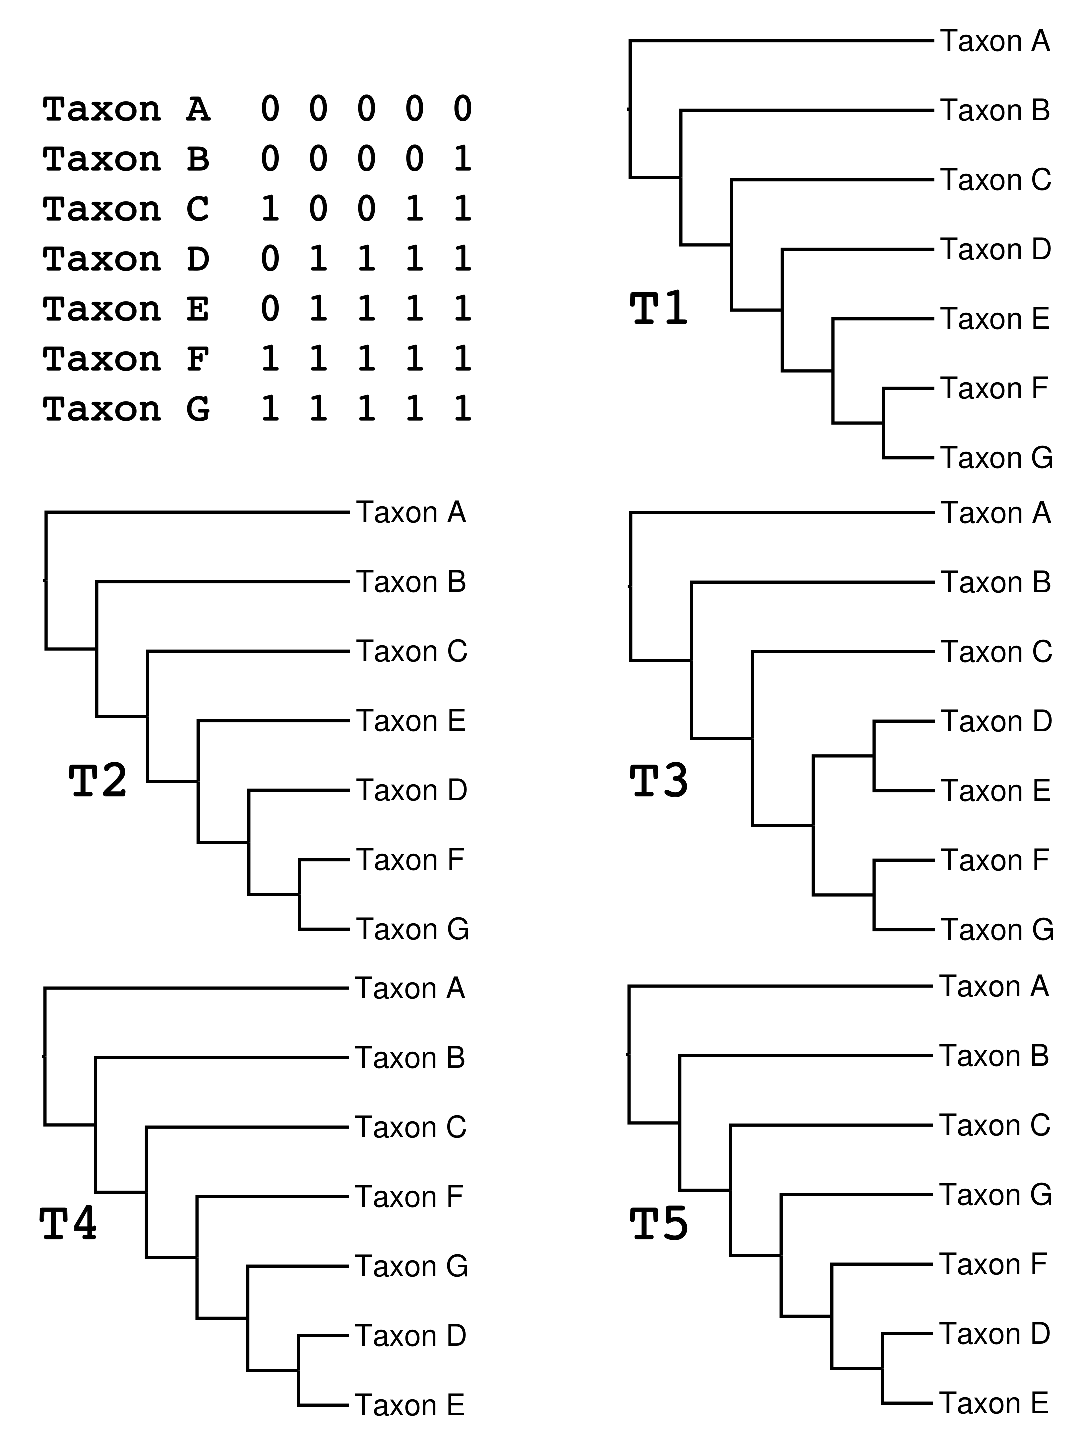
\includegraphics[scale=0.75]{figures/tut5/coddington_and_scharff_col0_trees.eps}}
	{\caption[\textcite{Coddington_and_Scharff_1994} exemplo]{Matriz da Tabela 1 de \textcite{Coddington_and_Scharff_1994} e 5 topologias obtidas em TNT por enumeração implícita e opção de colapso de ramos \texttt{collapse 0}.}\label{tut5:fig:optimization}} 
  \end{figure}

%%%%%%%%%%%%%%%%%%%%%%%%%%% FIM DA FIGURA OPTIMIZATION %%%%%%%%%%%%%%%%%%%%%

Após ter concluida a otimização destes caracteres nestas topologias você deverá verificar se você optimizou corretamente. Para isso, há dois arquivos disponíveis no diretório deste tutorial: \texttt{exercicio\_5.2\_matrix.tnt} e \texttt{exercicio\_5.2\_trees.tre}, que se referem à matriz e topologias apresentadas na Figura \ref{tut5:fig:optimization}. O comando de TNT que permite a reconstrução de caracteres em determinada topologia é o comando ``\texttt{recons}''. Inicie o TNT e digite ``\texttt{help recons}''. Você deverá obter:

\texttt{tnt*>help recons}\\
\texttt{RECONS}\\
\texttt{~~~~N/L;    most parsimonious reconstructions for character(s) L, tree(s) N}

Portanto, o comando ``\texttt{recons 0/1}'' apresentaria a(s) recontrução(ões) do caráter 2 na topologia 1 da Figura \ref{tut5:fig:optimization}. Se você executar ``\texttt{recons}'' todas as reconstruções possíveis para todos os caracteres e topologias serão apresentadas. Finalmente, se você executar ``\texttt{recons /0}'', todas as recontruções do caráter 1 serão apresentadas em todas as topologias.

A apresentação das reconstruções em TNT obedece o formato ilustrado na Figura \ref{tut5:fig:recons}. A numeração nos nós referem-se ao estado de caráter estimado para o caráter de acordo com a reconstrução. Arestas cujos vértices possuem estados distintos indicam transformação de estados de caráter. Observe que em alguns casos (veja Figura \ref{tut5:fig:recons}) há mais do que uma reconstrução para um determinado caráter dado uma topologia. Neste caso em particular, a primeira reconstrução (\texttt{reconstruction 0}) foi executada pelo algoritmo de DELTRAN (de \textit{delayed transformation}) ao passo que a segunda  (\texttt{reconstruction 1}) pelo algoritmo de ACCTRAN (de \textit{accelerated transformation}) \parencite{Farris_1970, Swofford_and_Maddison_1987}. Quando há mais do que uma reconstrução possível e igualmente parcimoniosas, a otimização do caráter é ambígua \parencite{Farris_1970} e baseado no critério de otimização não há justificativa para selecionar uma ou outra. O TNT é o único programa que apresenta todas as reconstruções possíveis para determinado caráter dado uma topologia utilizando ACCTRAN e DELTRAN ou a combinação dos dois algoritmos. Alguns autores, por exemplo \textcite{dePinna_1991}, argumentam que ACCTRAN seria defensável filosoficamente, argumentos que são rejeitados por \textcite{Agnarsson_and_Miller_2008}. Para uma revisão sobre o assunto consulte \textcite{Agnarsson_and_Miller_2008}.

Observe se para as otimizações que você fez à mão havia uma outra alternativa e anote nas topologuias da Figura \ref{tut5:fig:optimization}.

%%%%%%%%%%%%%%%%%%%%%%%%%%% FIGURA RECONS TNT %%%%%%%%%%%%%%%%%%%%%%%%%%%
%  \vspace{-1em}
  \begin{figure}[H]
    %\ffigbox[\FBwidth]
       \centering
      {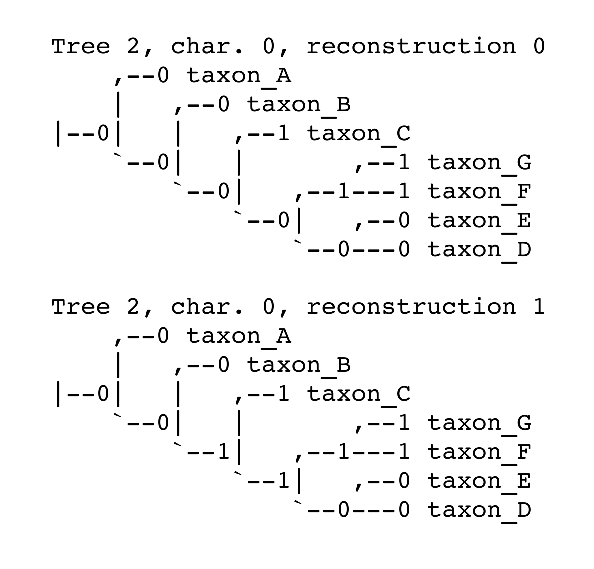
\includegraphics[scale=0.70]{figures/tut5/reconstrucao_tnt.eps}}
	{\caption[\textcite{Coddington_and_Scharff_1994} reconstrução]{Otimização do caráter 1 na Topologia 3 da Figura \ref{tut5:fig:optimization} seguindo \textcite{Coddington_and_Scharff_1994}.}\label{tut5:fig:recons}} 
  \end{figure}

%%%%%%%%%%%%%%%%%%%%%%%%%%% FIM DA FIGURA RECONS TNT %%%%%%%%%%%%%%%%%%%%%

\stepcounter{ex}
\begin{blackBlock}{\textbf{Exercicio 5.\arabic{ex}}}\label{tut4:ex:5.3}

Agora que você já conhece um pouco da teoria, vamos examinar duas regras de colapso de ramos existentes em TNT. Os comandos ``\texttt{collapse}'' e ``\texttt{help collapse}'' lhe fornecem a opção de \textit{default} de TNT para este comando e as opções disponíveis no programa, respectivamente. Iremos explorar duas destas opções, uma vez que são as mais comumente utilizadas na literatura e respondem por possíveis diferenças entre os resultados apresentados por TNT e PAUP*.

\end{blackBlock}


  \begin {myindentpar}{0.3cm}
  \begin{enumerate}[\itshape i.]
	\item{Utilizando a configuração original de TNT, faça uma busca por enumeração implícita, imprima as tolopogias no terminal e, com referência àqueles ilustradas na Figura \ref{tut5:fig:optimization} responda:}
	  \begin {myindentpar}{0.5cm}
	  \begin{enumerate}[\itshape a.]
		\item{Quais tolopogias foram recuperadas? Considere que as topologias apresentadas na Figura \ref{tut5:fig:optimization} são binárias ao passo que as apresentadas após a análise tiveram seus ramos colapsados, verifique quais topologias binárias são compatíveis com as da Figura \ref{tut5:fig:optimization}.}
			\begin{center}
			\line(1,0){400}\\
			\end{center}
		\item{Baseada nas reconstruções dos caracteres, você poderia explicar qual regra esta sendo adotada para colapsar os ramos?}
			\begin{center}
			\line(1,0){400}\\
			\line(1,0){400}\\
			\line(1,0){400}\\
			\end{center}
	  \end{enumerate}
	  \end{myindentpar}
	\item{Modifique a regra de colapso adotando aquela que é \textit{default} em PAUP*, execute novamente a análise e responda:}
	  \begin {myindentpar}{0.5cm}
	  \begin{enumerate}[\itshape a.]
		\item{Quais tolopogias foram recuperadas com essa nova regra?}
			\begin{center}
			\line(1,0){400}\\
			\end{center}
		\item{Baseada nas reconstruções dos caracteres, você poderia explicar qual regra esta sendo adotada para colapsar os ramos?}
			\begin{center}
			\line(1,0){400}\\
			\line(1,0){400}\\
			\line(1,0){400}\\
			\end{center}
		\item{Qual regra você adotaria em seu estudo? Justifique.}
			\begin{center}
			\line(1,0){400}\\
			\line(1,0){400}\\
			\line(1,0){400}\\
			\end{center}
	  \end{enumerate}
	  \end{myindentpar}
  \end{enumerate}
  \end{myindentpar}

\section{Diagnoses}\label{tut5:apo}
	Neste seção iremos explorar o comando ``\texttt{apo}'' do TNT e sua relação com o comando ``\texttt{recons}'' discutido no tópico anterior.\\
	O comando \texttt{apo} possui as seguintes opções:\\
\texttt{tnt*>help apo;}\\
\texttt{APO}\\
\texttt{~~~~N~~~~~plot synapomorphies for tree(s) N }\\
\texttt{~~~~[N~~~~plot synapomorphies common to tree(s) N }\\
\texttt{~~~~-~~~~~list instead of plotting on tree }\\
\texttt{~~~~[-N/L~list synapomorphies common to tree(s) N, node(s) L }\\

Considere a matrix no arquivo \texttt{vertebrados.tnt}. A análise cladística por enumeração implícita gera três topologias (\texttt{Tree 0 - Tree 2} da Figura \ref{tut5:fig:apo_vert}).

%%%%%%%%%%%%%%%%%%%%%%%%%%% FIGURA VERTEBRADOS TREES %%%%%%%%%%%%%%%%%%%%%%%%%%%
%  \vspace{-1em}
  \begin{figure}[H]
    %\ffigbox[\FBwidth]
       \centering
      {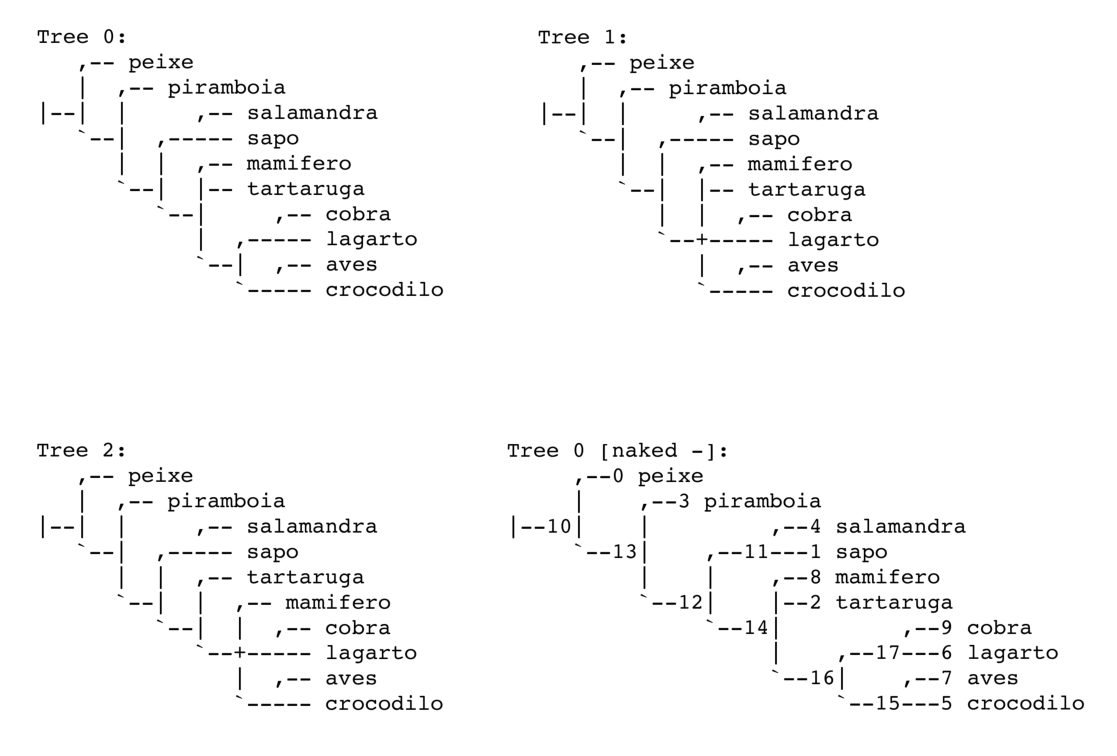
\includegraphics[scale=0.80]{figures/tut5/vertebrate_trees.eps}}
	{\caption[Enumeração implícita de \texttt{vertebrados.tnt}]{Topologias (\texttt{Tree 0 - Tree 2}) resultantes da enumeração implícita de \texttt{vertebrados.tnt}. A topologia ``\texttt{Tree 0 [naked -]}'' foi impressa com a opção do comando ``\texttt{naked}'' de TNT que apresenta a numeração dos nós na Topologia \texttt{0}.}\label{tut5:fig:apo_vert}}
  \end{figure}

%%%%%%%%%%%%%%%%%%%%%%%%%%% FIM DA FIGURA VERTEBRADOS TREES %%%%%%%%%%%%%%%%%%%%%

Há duas formas de visualizar as sinapomorfias não ambíguas para essas tolologias. A primeira delas é impressa na topologia pelo comando, por exemplo, \texttt{apo 0} -- que apresenta as apomorfias inequívocas para a topologia \texttt{Tree 0} (veja Figura \ref{tut5:fig:apo_tree0}). Outra forma de apresentar as sinapomorfias é listando-as com o comando, por exemplo, ``\texttt{apo- 0}'' -- que lista as apomorfias inequívocas para a topologia \texttt{Tree 0} (veja Figura \ref{tut5:fig:apo_tree0}). Observe que neste último caso, é conveniente referenciar os nós da topologia utilizando o comando ``\texttt{naked-}'' antes de executar ``\texttt{tplot}'' (consulte o \textit{help} para esses dois comandos noa TNT).


%%%%%%%%%%%%%%%%%%%%%%%%%%% FIGURA VERTEBRADOS APO 0 %%%%%%%%%%%%%%%%%%%%%%%%%%%
%  \vspace{-1em}
  \begin{figure}[H]
    %\ffigbox[\FBwidth]
       \centering
      {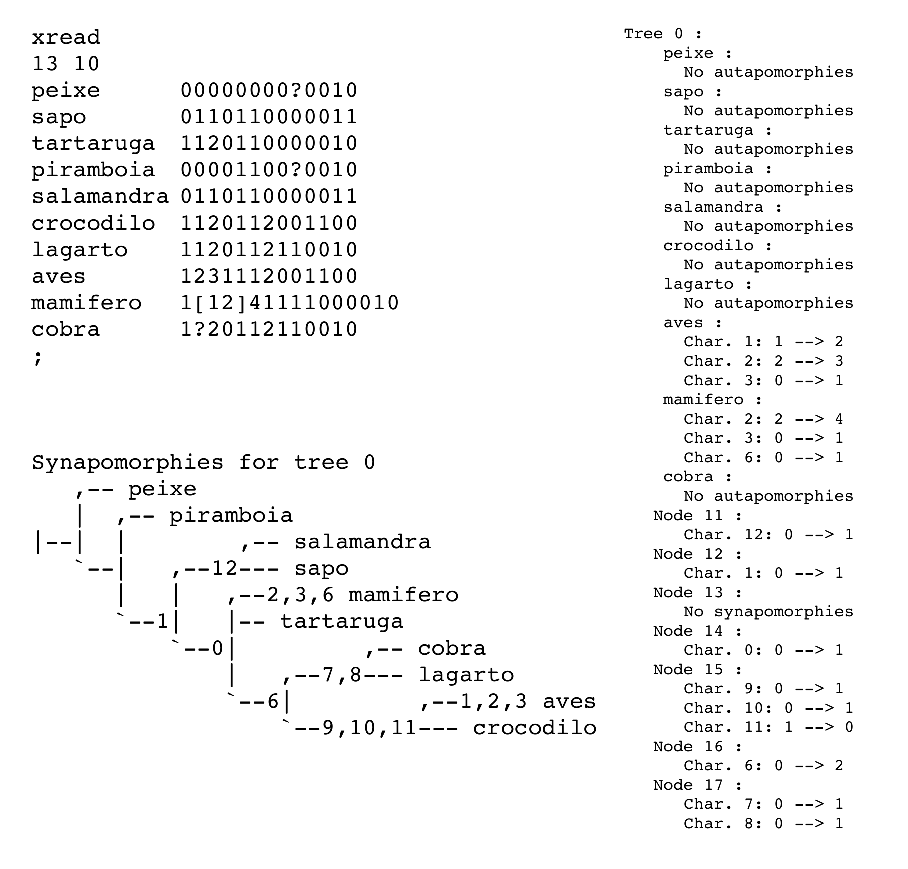
\includegraphics[scale=0.80]{figures/tut5/vertebrados_apo_tree_0.eps}}
	{\caption[Apomorfias para \texttt{Tree 0} em \texttt{vertebrados.tnt}]{Matriz de dados \texttt{vertebrados.tnt} e apomorfias para \texttt{Tree 0} plotadas na topologia e listadas.}\label{tut5:fig:apo_tree0}} 
  \end{figure}

%%%%%%%%%%%%%%%%%%%%%%%%%%% FIM DA FIGURA RECONS APO 0 %%%%%%%%%%%%%%%%%%%%%


\stepcounter{ex}
\begin{blackBlock}{\textbf{Exercicio 5.\arabic{ex}}}\label{tut4:ex:5.4}
	Os exercícios abaixo são referêntes à matriz de dados em \texttt{vertebrados.tnt}.
\end{blackBlock}


  \begin {myindentpar}{0.3cm}
  \begin{enumerate}[\itshape i.]
	\item{Na figura abaixo, indique as apomorfias comuns para as topologias \texttt{Tree 0 --2}.}
%%%%%%%%%%%%%%%%%%%%%%%%%%% FIGURA VERTEBRADOS COMMOM APO %%%%%%%%%%%%%%%%%%%%%%%%%%%
%  \vspace{-1em}
  \begin{figure}[H]
    %\ffigbox[\FBwidth]
       \centering
      {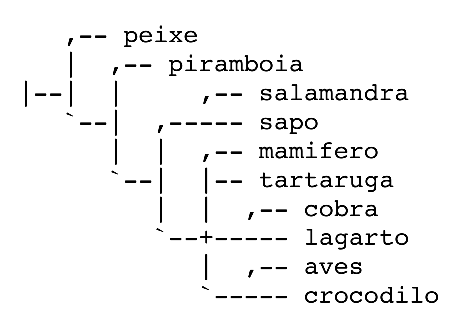
\includegraphics[scale=1.00]{figures/tut5/vertebrados_trees_consenso.eps}}\label{tut5:fig:apo_common} 
	%{\caption[Apomorfias comuns para \texttt{vertebrados.tnt}]{Matriz de dados \texttt{vertebrados.tnt} e apomorfias para \texttt{Tree 0} plotadas na topologia e listadas.}
  \end{figure}

%%%%%%%%%%%%%%%%%%%%%%%%%%% FIM DA FIGURA RECONS COMMOM APO %%%%%%%%%%%%%%%%%%%%%
	\item{Qual é a polarização dos caracteres que sustentam a hipótese de que Aves e Crocodilos são grupos irmãos nas topologias \texttt{Tree 0 --2}?}

	   \line(1,0){400}\\
	   \line(1,0){400}\\
	   \line(1,0){400}\\

	\item{Quais são as possiveis reconstruções do caráter 6 nas tolopogias \texttt{Tree 0 --2}? (inicio da contagem no zero)}

	   \line(1,0){400}\\
	   \line(1,0){400}\\
	   \line(1,0){400}\\

	\item{Por que não há sinamoporfia(s) listadas para o nó 13 das tolopogias \texttt{Tree 0 --2} e mesmo assim ele é resolvido nestas hipóteses?}

	   \line(1,0){400}\\
	   \line(1,0){400}\\
	   \line(1,0){400}\\


  \end{enumerate}
  \end{myindentpar}
%%%%%%%%%%%%%%%%%%%%%%%%%%%% HERE ENDS TEXT AND ADDS REFERENCES %%%%%%%%%%%%%%%%%%%%%%%%%%%% 
\section{Referências}\label{tut5:refs}
\printbibliography[heading=none]
\end{refsection}
%

